\chapter{Literature Review}
\label{chap:lit-review}

\section{Introduction}

\section{Drones}

\subsection{Modelling}

When designing a control system, arguably the most crucial part of the process is to derive an accurate mathematical model of the plant that is to be controlled. The plant in this case is a unmanned aerial vehicle (UAV) in a `quadcopter' configuration. 

As part of the X-4 Flyer project,~\cite{hamel2002dynamic} set out to derive a simple model for their plant using only rigid body dynamics and abstract force and torque actuators. As stated by~\cite{Pounds2010c}, this model, like many others that were derived at the time, represents the quadcopter as a rigid body mass with inertia and autogyroscopics, affected only by gravity and actuator torques.~\citeauthor{Pounds2010c} further argues that these simple quadcopter models do not accurately represent the complex helicopter-like behaviour exhibited by real quadcopters at high rotor speeds. These high-speed rotor effects include the blade flapping effect, which affect the quadcopter frame's oscillatory modes, rotor flapping from varying quadcopter yaw angles, and variable airflow velocities over the rotor blades from varying roll and pitch angles.

In an attempt to create a quadcopter model that will allow a quadcopter to be more accurately controlled at high rotor speeds,~\citeauthor{Pounds2010c} set out to derive a model incorporating the rigid body dynamics, as well as the aerodynamic effects mentioned earlier. Their model is based on the diagram given in Figure~\ref{fig:chap2-quad-model}.

\begin{figure}
  \centering
  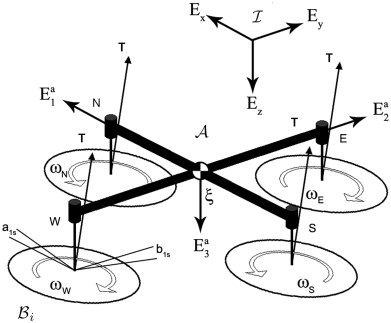
\includegraphics[width=0.5\textwidth]{figures/chapter2/pounds_quad-model.jpg}
  \caption[A diagram of the quadcopter model, including the blade flapping dynamics.]{A diagram of the quadcopter model, including the blade flapping dynamics. Adapted from~\cite{Pounds2010c}.}
\label{fig:chap2-quad-model}
\end{figure}

Their resulting model was used to develop a simple hovering Proportional Integral Differential (PID) attitude and altitude controller for the purpose of model verification. The results show that the drone stabilised itself in indoor flight with $\pm1$\textdegree of precision and $\pm5$\textdegree of precision during outdoor flight. The lower precision during outdoor flights is due to the added wind disturbances, etc. Thus, the model, as it stands, is sufficiently accurate to safely control a drone for hovering. However, they did not compare their model, which includes aerodynamic effects, against the model of~\citeauthor{hamel2002dynamic}, which is based on rigid body dynamics. 

\subsection{Control}

\subsubsection{Introduction}

After an accurate model, the next most important part of a good control system is the controller itself. Many controllers have been implemented and tested on quadcopters over the years. Different control strategies have also been investigated. Some of the most prevalent control strategies and controllers are discusses.

\subsubsection{Indoor vs. Outdoor Control}

There are different types of quadcopters, each of them equipped with different sensors and equipment. The two main types of quadcopters are indoor and outdoor quadcopters. Each of them work in different ways and implement very different control schemes. 

Indoor drones may or may not come equipped with an on-board inertial measurement unit (IMU), which includes an accelerometer and gyroscope, for stability control. However, they commonly rely soley an external motion detection system which tracks the drones movements, providing position and rotation (also known as pose) feedback to controller, thereby closing the control loop. These drones are exceptionally accurate and capable of performing remarkable acrobatic feats. However, they are restricted to carefully controlled indoor environments.

Outdoor drones, without the luxury of having very accurate external sensors available, have to rely on their on-board sensors to provide the controller with pose feedback. These on-board sensors these drones come equipped with may vary between quadcopter platforms, however they almost certainly come equipped with an IMU to provide pose data. However, since the IMU readings for position data drifts with time due to integration errors, a global positioning system (GPS) sensor is added to provide a base-line reading for a quadcopter's position. Other sensors that may be included are magnetometers, barometers, visual feedback sensors and sonar sensors. To combine the readings of the different sensors, a filtering technique, such as the Extended Kalmann Filter, is used. The pose error of the combination of the different readings are, in theory, less than the most accurate sensor in the suite, but this has not yet been proven. 

\subsubsection{Hovering Control}

Stable hovering of a quadcopter has been the focus of many projects and research papers in the past 15 years. As a result, many different control methods and schemes have been investigated, implemented and compared. Hovering control refers to a quadcopters ability to hover and remain stable at a set point in 3-dimensional space.

\cite{bouabdallah2004pid}, as part of their `OS4' project, compared the modern linear quadratic regulator (LQR) and classic PID controller with one another, with respect to the control performance (disturbance rejection, reference tracking, etc.), of a quadcopter.

They found that the PID controller produced better results than the LQR in terms of reference tracking and dynamic performance. This was a surprising result, since LQR controllers normally excel at controlling unstable, underactuated plants such as a quadcopter platform. They suspect that the reason for this result may be because they neglected the effects of actuator dynamics, such as blade and rotor flapping, in their drone model. However, they do expect that an LQR controller will produce superior results if these effects are taken into account. 

Some researchers have also investigated controlling a drone using an H-infinity (H$_{\inf}$) control structure and a model predictive controller (MPC).

Most notably,~\cite{raffo2010integral} have done extensive research on this topic. MPC's are computationally efficient and modern controllers that drive a plant's state to a reference state within predefined constraints (eg.\ motor saturation, model dynamics, etc.), while a properly designed non-linear H$_{\inf}$ controller is very good at rejecting disturbances (eg.\ wind gusts, motor vibrations, etc.) and are robust to model uncertainties. They opted to combine the two controllers in an intelligent manner in order to extract the most efficient performance out of their drone. 

In their simulations they found that the resulting controller performed admirably, presenting good reference tracking, proving to be robust with uncertain mass and inertia terms and deals well with disturbances on all 6 degrees of freedom at different points in time. However, they are yet to implement and test their controller configuration on a real drone. Although the algorithms and methods they used are computationally efficient, it may still prove to be too computationally intensive for the limited computing power on-board a drone. Given the fast growth of processing power, however, this controller configuration may become a more viable option in the near future. 

Controllers for enabling a drone to hover have already been successfully designed and implemented, and it is therefore possible to accurately control a drone during hovering operations. 

\section{Computer Vision}

\subsection{Introduction}

Computer vision is a diverse field which primarily focuses on devising methods for acquiring, processing, analysing and understanding images captured of the real world. There are various sub-fields of research, but a common theme across all the fields is to mimic the human ability to perceive and understand an image, and perhaps react accordingly to different visual inputs. 

The fields of interest for this thesis, is the object detection, tracking and pose estimation fields. This section aims to discuss the work that has been done in these fields. 

\subsection{Camera Matrix}

An image is a collection of 2-dimensional vectors representing a collection of 3-dimensional space vectors. These collections of vectors are related by a matrix $C$, known as the camera matrix. The camera matrix contains the intrinsic parameters of the camera that recorded the image, i.e.\ the focal lengths and principle point of the image, as well as the extrinsic parameters of the camera, i.e.\ the translation and rotation information. The camera matrix $C$ given is given by Equation~\ref{eq:cam-matrix}, as derived by~\cite{heikkila1997four}. 
\begin{equation}
  \label{eq:cam-matrix}
  C = 
  \begin{bmatrix}
    f_x & 0   & u_0 \\
    0   & f_y & v_0 \\
    0   & 0   & 1   \\
  \end{bmatrix}
  \begin{bmatrix}
    R | T
  \end{bmatrix}
\end{equation}

where $f_x$ and $f_y$ describe the focal lengths of the camera, and $u_0$ and $v_0$ are the principal points. $R$ is a $3\times3$ matrix describing the rotation of the camera, and $T$ is a three-dimensional vector describing the translation of the camera. 

If the camera matrix $C$ is known, the 3-dimensional coordinates for any 2-dimensional image can be determined by the relation given in Equation~\ref{eq:2d-to-3d}. The camera matrix is commonly determined through some camera calibration procedure. One such a procedure is discussed in Section~\ref{sec:chap2-cam-calibration}.

\begin{equation}
   \label{eq:2d-to-3d}
   \begin{bmatrix}
     x_c & y_c & 1 \\
   \end{bmatrix}^T
   = C
   \begin{bmatrix}
     x_w & y_w & z_w & 1 \\
   \end{bmatrix}^T
 \end{equation}

\subsection{Camera Calibration}
\label{sec:chap2-cam-calibration}

There are various camera calibration procedures available, from the two-step calibration described by~\cite{melen1994geometrical} to the classical approach given by~\cite{slama1980manual}, where a nonlinear error function is minimised. However, the minimisation problem presented by~\citeauthor{slama1980manual} is computationally inefficient and slow, while~\citeauthor{melen1994geometrical}'s method does not account for image distortion and correction.

A popular calibration method, as used by the OpenCV computer vision library [\cite{bradski2000opencv}], is the four-step method, proposed by~\cite{heikkila1997four} as an extension to the two-step method which was the prevalent at the time.

\subsection{Principle n-Points Problem}

\subsection{Random Sample Consensus}

\section{Machine Learning Algorithms}

\subsection{Introduction}
